\section{Hardware/Software mapping}%
\label{sec:hw-sw-mapping}
In the hardware/software mapping activity, the functionality associated to a
software component is mapped to the hardware responsible for executing it. It is
represented by a UML deployment diagram used to depict the relationship between
run-time components and nodes.
Components are self-contained entities that
provide services to other components or actors, e.g., the \texttt{RVVS\_App} in
Fig.~\ref{fig:deployment-diag}.
A node is a physical device or an execution environment in which components are
executed, such as a desktop computer, or \texttt{myLinux} in Fig.~\ref{fig:deployment-diag}, represented by boxes containing
component icons. Furthermore, a node can contain another node, for example a
device can contain an execution environment such as virtual machine.

The UML deployment diagram for the \gls{rfcar} system is depicted in
Fig.~\ref{fig:deployment-diag}, where the two nodes --- Smartphone and LinuxVM
--- are represented in turquoise and orange, respectively. The ball-and-socket
joint identifies the provided and required interfaces, respectively. Thus, the
\texttt{RVVS\_app} provides wireless communication interfaces that the
\texttt{Android\_app} can use, namely Wi-Fi and GPRS~.
Furthermore, it highlights the client-server software pattern, with the
\texttt{RVVS\_app} and \texttt{NVS\_app} serving the requests (servers) that the
\texttt{Android\_app} requests (client).
The \texttt{Android\_app} communicates with the \texttt{NVS\_app} via Bluetooth,
or, if the communications fail, through any of the available communications
channels for the \texttt{RVVS\_app} that forwards that request for
\texttt{NVS\_app}.

Lastly, it should be noted that in a real-world scenario the \texttt{NVS\_app}
and \texttt{RVVS\_app} are mapped to a different hardware, which is also distinct
between them, e.g., the former in an \texttt{STM32} and the latter in a
\texttt{Raspberry Pi}. However, in the virtualized environment, and ideally,
they represent two distinct processes that must communicate via an \gls{ipc}
mechanism, e.g., sockets. Nonetheless, to ease and speed up the development it
is perfectly acceptable to implement both processes into the same application in
the early development phase.
% Deployment diagram
\begin{figure}[!hbt]
\centering
    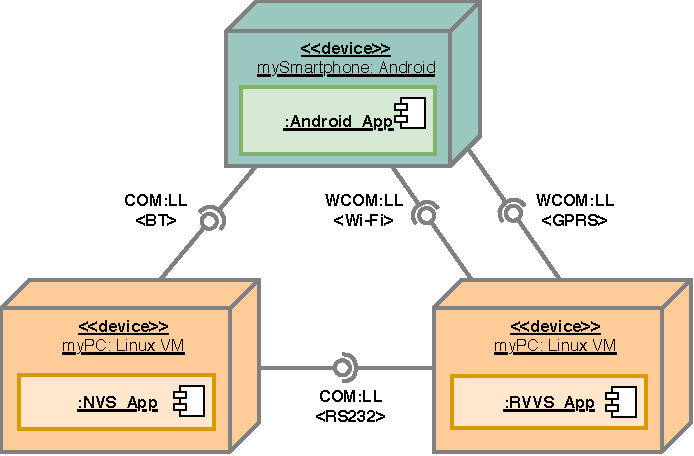
\includegraphics[width=0.55\textwidth]{./img/deployment-diag.pdf}
  \caption{\acrshort{rfcar} Deployment diagram}%
\label{fig:deployment-diag}
\end{figure}
%
%%% Local Variables:
%%% mode: latex
%%% TeX-master: "../../../dissertation"
%%% End:
